\section{\ref{PS:Q:Availability}}

\textit{Can we create a solution where removing one or more nodes from the system at runtime does not cause system failure?}\newline\newline

\noindent To answer whether or not a fully decentralized current Siemens system can handle removing one or more nodes at runtime, the discussion section of this experiment also contains a discussion with regards to the components analyzed in \cref{cha:stateOfTheArt}: \nameref{cha:stateOfTheArt}.\todo{Why the chapter name ref?}

\subsection{Experiments}
The \ref{PS:Q:Availability} problem address if the proposed decentralized solution is able to continue its functions even though nodes are interrupted and removed from the system at runtime.
The proposed decentralized solution should be able to continue maintaining the global setpoint of the wind farm even if some turbines become unavailable, assuming that the needed production capacity is available.

The below experiment is repeated with $N = 1, 5, 10, 15$ failing turbines of 30 running turbines.
%
The experiment has the following procedure:
\begin{enumerate}
	\item Start the system with 30 turbines.
	\item Make sure the system is stable.
	\item Kill N nodes.
\end{enumerate}

Did the system adjust the setpoints for all turbines to maintain the global setpoint?

\subsection{Results}
\label{sec:res:availability}
The plots in \cref{fig:exp:availability_kill15,fig:exp:availability_kill10,fig:exp:availability_kill5,fig:exp:availability_kill1} show how the decentralized solution reacts when killing 1, 5, 10 and 15 turbines. The figures are Matlab screen shots from the graphical interface presented in \cref{sec:graphicalInterface}. The x-axis show time in seconds and the y-axis show kW production. The global setpoint is set to 20,000~kW instead of 2000~kW for the experiment with 1 failing turbine is removed (\cref{fig:exp:availability_kill1}). The global setpoint value for this experiment has been set this high to provide a better visual representation for the case where 1 turbine has failed. 
% (a change of $globalSetpoint/nTurbines=2,000kW/30=66,6kW$ is harder to see than change of $20,000kW/30=666,6kW$). 
For the remainder of the cases (meaning where 5, 10 and 15 turbines are crashed), the global setpoint is set to 2000~kW.
The turbines are all running with a cycle time of 20 ms throughout this experiment.

\clearpage
\Cref{fig:exp:availability_kill1} shows an increase of production pr. turbine by approximately 20 kW pr. remaining turbines, after a single turbine is crashed. A global setpoint of 20,000kW was set for this test.

\begin{figure} [!h]
	\centering
	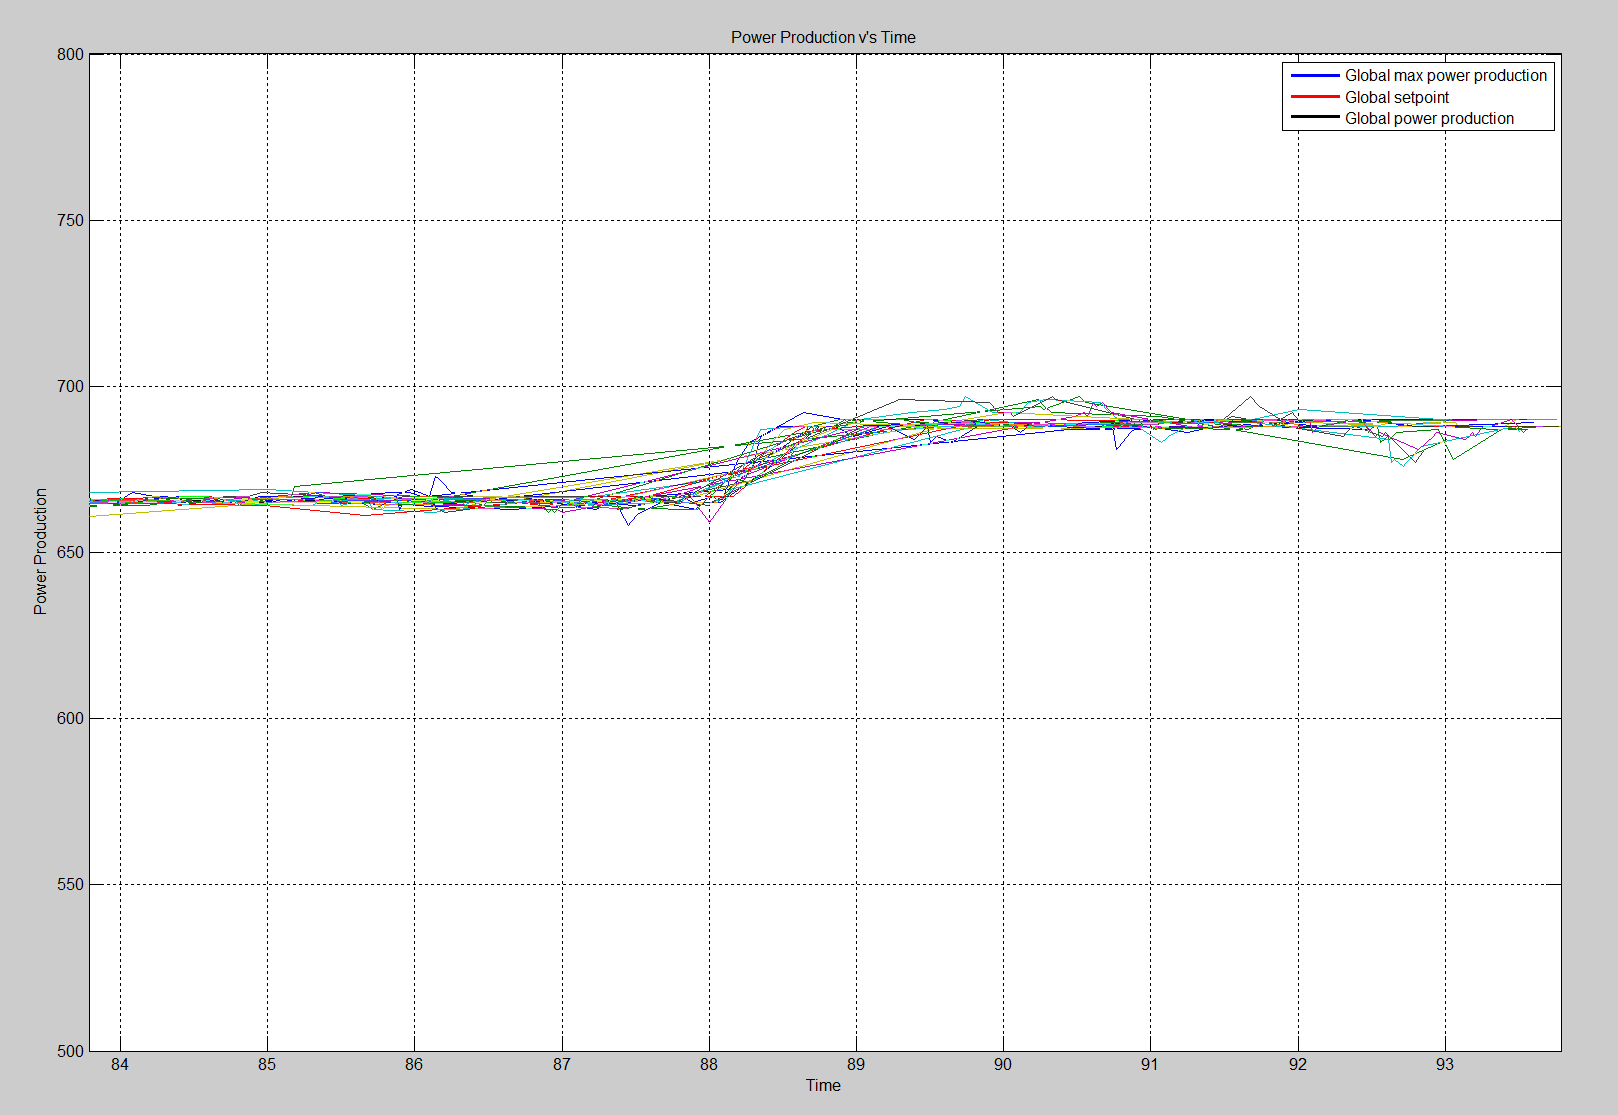
\includegraphics[width=\resultsFigureWidthScale\textwidth]{figures/Results/availabilitytest30-29_setpoint_20000.PNG}
	\caption{Availability test kill 1 out of 30 turbines}
	\label{fig:exp:availability_kill1}
\end{figure}

\Cref{fig:exp:availability_kill5} shows an increase of production pr. turbine by approximately 15 kW pr. remaining turbines, after 5 turbines are crashed. A global setpoint of of 2000kW was set for this test.

\begin{figure} [!h]
	\centering
	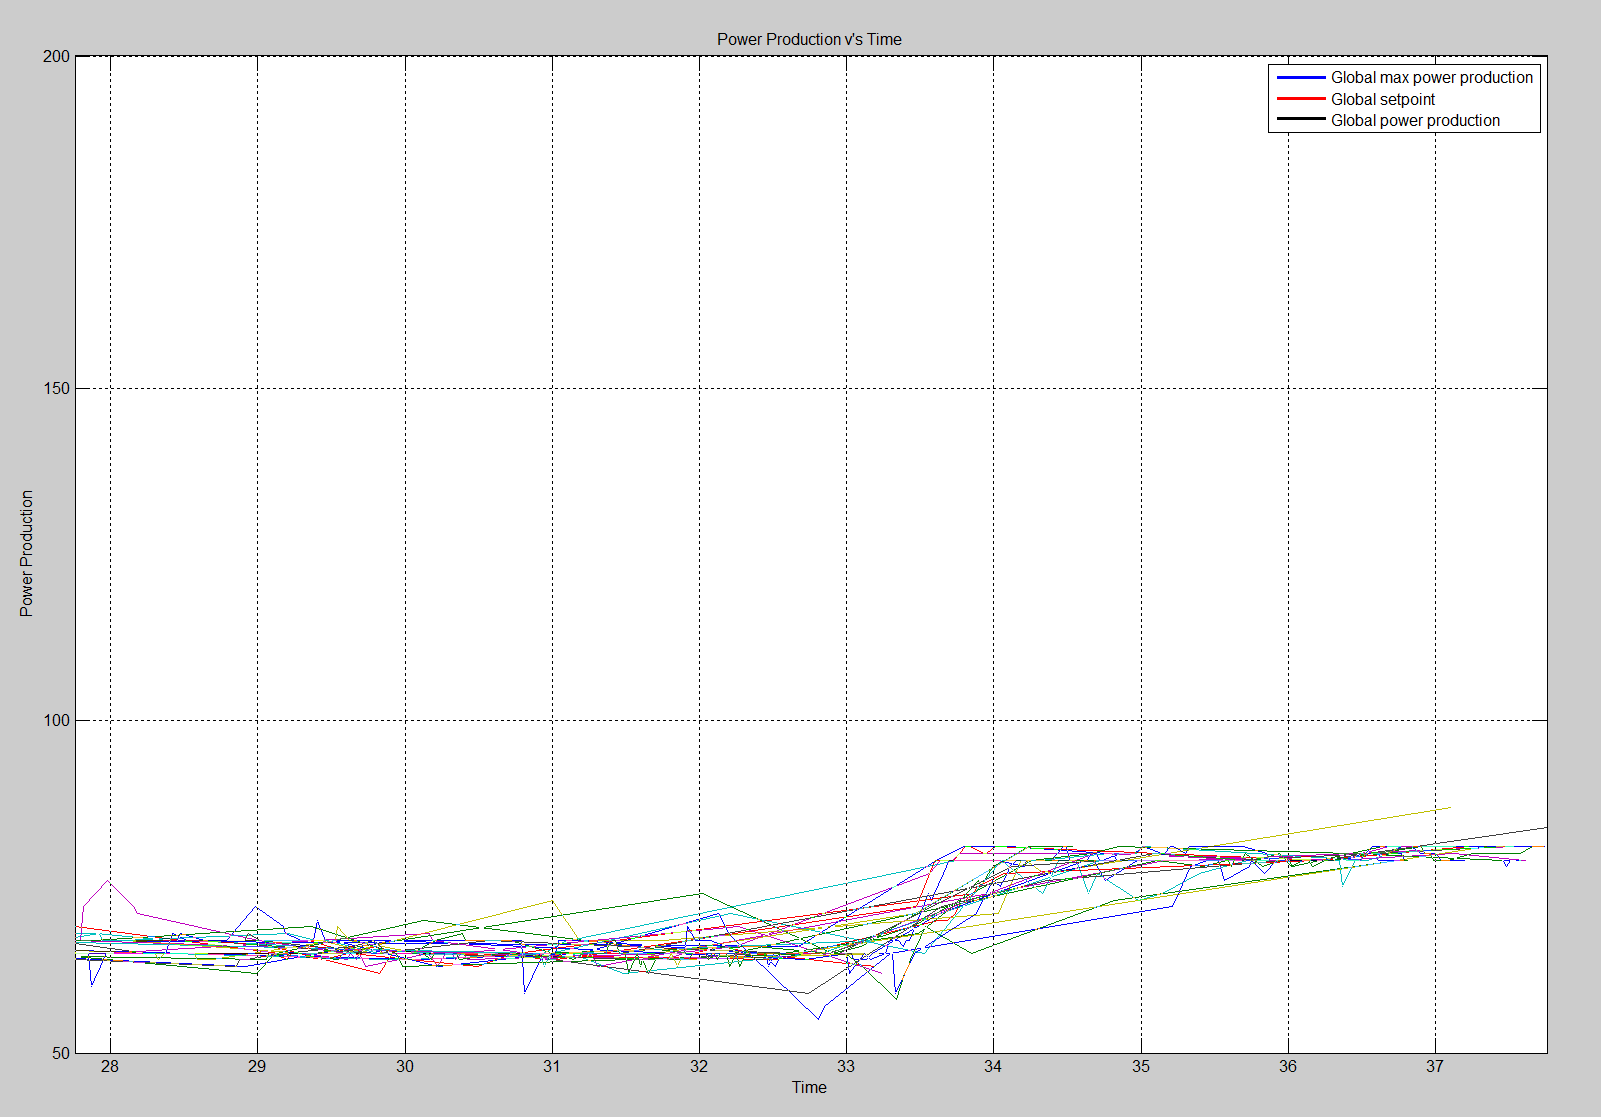
\includegraphics[width=\resultsFigureWidthScale\textwidth]{figures/Results/availabilitytest30-25_setpoint_2000.PNG}
	\caption{Availability test kill 5 out of 30 turbines}
	\label{fig:exp:availability_kill5}
\end{figure}

\FloatBarrier
\Cref{fig:exp:availability_kill10} shows an increase of production pr. turbine by approximately 30 kW pr. remaining turbines, after 10 turbines are crashed. A global setpoint of of 2000kW was set for this test.

\begin{figure}[!h]
	\centering
	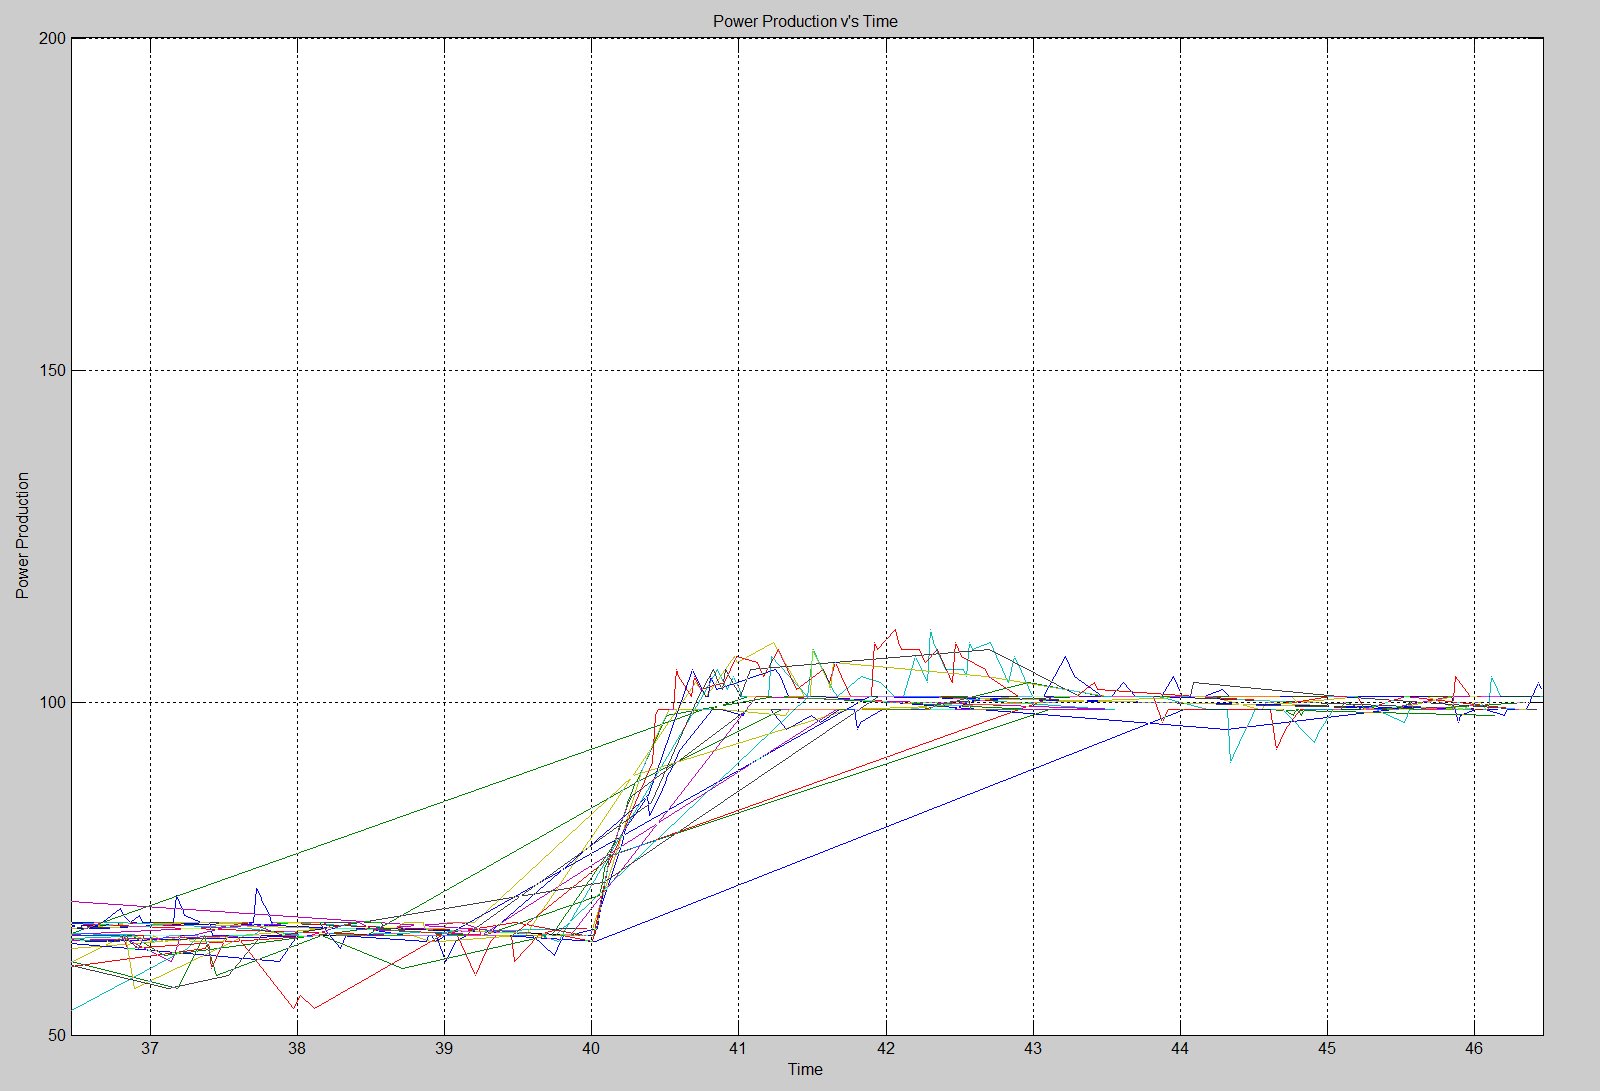
\includegraphics[width=\resultsFigureWidthScale\textwidth]{figures/Results/availabilitytest30-20_setpoint_2000.PNG}
	\caption{Availability test kill 10 out of 30 turbines}
	\label{fig:exp:availability_kill10}
\end{figure}

\FloatBarrier
\Cref{fig:exp:availability_kill15} shows an increase of production pr. turbine by approximately 60 kW pr. remaining turbines, after 15 turbines are crashed. A global setpoint of of 2000kW was set for this test.

\begin{figure}[!h]
	\centering
	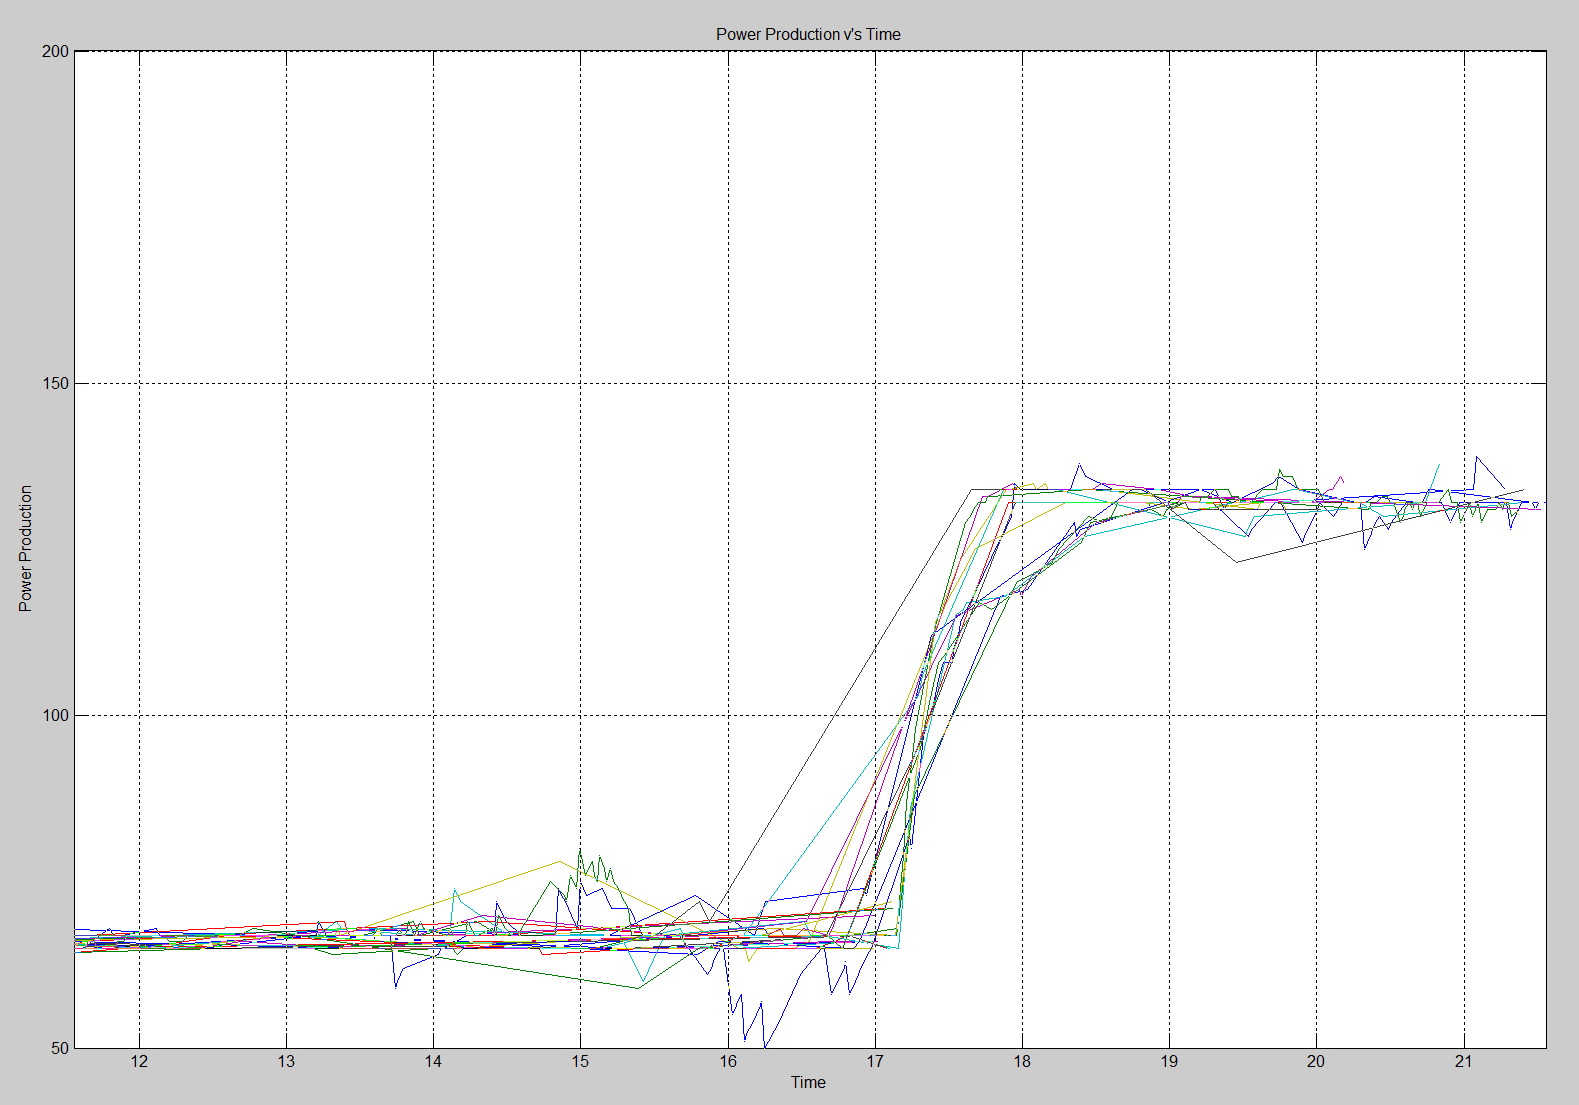
\includegraphics[width=\resultsFigureWidthScale\textwidth]{figures/Results/availabilitytest30-15_setpoint_2000.PNG}
	\caption{Availability test kill 15 out of 30 turbines}
	\label{fig:exp:availability_kill15}
\end{figure}

\FloatBarrier

The 'glitches' on the figures, where the plots shows several seconds between some of the data points, are caused by the eventhandler in Matlab handling events from DDS Blockset for Simulink (described in \cref{sec:graphicalInterface}). The eventhandler appears to be neglecting some of the events caused by the publication of turbine states, thus resulting in several seconds time interval between two data points. For the purpose of this experiment we are able to clearly see that it does the regulation, however the time frame is inaccurate.\todo{Shouldn't this be in discussion}
%(and any of the other experiments for that matter), this is acceptable since the tool is only used to provide a run-time GUI overview of the system.

\subsection{Discussion}
One of the main challenges of decentralized systems is to continue operation in the event of node failure of communication failure or node loss. As presented in  \cref{fig:exp:availability_kill15,fig:exp:availability_kill10,fig:exp:availability_kill5,fig:exp:availability_kill1} the decentralized solution can handle the loss of turbines. A turbine is considered offline if it does not publish any new data to any other turbines within a 150 ms timespan, defined by the Lifespan QoS parameter of the DataWriter described in \cref{sec:decen:ddsconf}.
This upper limit of 150 ms is chosen because 150 ms is the upper limit of the regulation cycle time in the current Siemens system.
% % % I am HERE Krause
After turbines have been detected caused by a node failure the remaining turbines in the wind farm will share the load of the missing turbines, to keep the global power production of the wind farm as close to the global setpoint as possible.

Let k = the number of turbines crashed, p = production of the crashed turbine, and n = number of remaining turbines. The expected increase of production pr. turbine when one or more turbines are crashed, is denoted as (by regulation algorithm definition explained in \cref{sec:calculateSetpoints}): $$Production~increase~per~turbine = \frac{\sum\limits_{i=1}^k(p)}{n}$$

Thus the expected production increase for the case where a single turbine is crashed (\cref{fig:exp:availability_kill1}) is: $$\frac{\sum\limits_{i=1}^1(666,6kW)}{29}\approx23kW$$

Hence for the rest of the cases (note that the global setpoint for these cases are 2000kW, thus the production of each turbine is 66,6 kW as apposed to 666,6 kW for the case where one turbine was crashed):
\newline\newline
\noindent5 turbines crashed (\cref{fig:exp:availability_kill5}) $$\frac{\sum\limits_{i=1}^5(66,6kW)}{25}\approx13kW$$

\noindent10 turbines crashed (\cref{fig:exp:availability_kill10}) $$\frac{\sum\limits_{i=1}^{10}(66,6kW)}{20}\approx33kW$$

\noindent15 turbines crashed (\cref{fig:exp:availability_kill15}) $$\frac{\sum\limits_{i=1}^{15}(66,6kW)}{15}\approx67kW$$

These expected values matches the increased productions shown in figures \ref{fig:exp:availability_kill5} to \ref{fig:exp:availability_kill15}. The glitches of the figures are caused by the simulated turbine data and is therefore accepted for the purpose of this experiment. Thus we conclude that the remaining turbines will share the extra load between themselves and continue power production, when a turbines crashed, as expected, which means removing one or multiple turbines from the system does not impede the regulation of the wind farm.

%The time it takes the decentralized solution to detect a turbine loss and recover power production is dependent on the following parameters:
%
%\begin{itemize}
%	\item Time of turbine loss detection, which is defined by the History QoS to 150 ms, $I$.
%	\item Time between regulation cycles, in the test cases presented in \cref{sec:res:availability} the time is set to 20 ms, $S$.
%	\item Time of calulation of a new setpoint, $C$.
%	\item Time for the turbine to regulate power production according to the new setpoint. In the turbines this process is simulated with a simple regulation that may take several regulation cycles to complete $R$.
%\end{itemize}
%
%Thus the time for recovery of the power production when a turbine failure occurs can be calculated as $T = I + S + C + R$ which translates to $150 ms + 20 ms + C + R = 170 + C + R ms$. This time can be reduced by lowering the time it takes to detect a turbine is offline which increases the likelihood of detecting a delayed turbine as offline, or by lowering the time between regulation cycles which increases the likelihood of cache reads.

The time it takes for the turbines to regulate according to crashed turbines are of course also an important factor. However since we are using an arbitrary regulation algorithm and turbine simulations, we cannot conclude anything with regards to this subject.

% The only thing we can conclude is that the turbines regulate according to multiple crashed turbines relatively fast, meaning that the time it takes for the turbines to regulate according to one or more crashes happens within an acceptable timeframe of 1 to 4 seconds. 

When it comes to availability for the a potential decentralized Siemens Wind Power wind farm, handling the communication for the regulation algorithm run by the Park Pilot is only one part of the picture. Availability for the decentralized Wind Park Supervisor, which handles external communication and data storage and aggregation, must also be addressed. 
To ensure that the wind farm is available to the outside world, in the face of turbine failures, sets special requirements to the component chosen to handle external communication. To handle this BLABLA \todo{KRAUSE} has been identified as the optimal component (as concluded in \cref{cha:resourceManagement}). This component can ... BLABLA \todo{KRAUSE}

To ensure available data storage, the problem of data loss when a turbine is unresponsive must be addressed. A turbine has several control and measurement points which are continually logged to a local data store. Should a turbine break down, the local data may be destroyed with the turbine. This sets special requirements to the component handling data storage. In \cref{sec:databaseStorage} the requirements to the data storage component is described and MongoDB was identified as the best choice to solve the availability problem of data storage. MongoDB is capable of automatic replication of data between turbines, such that data is still available should a turbine failure occur. As well as replication MongoDB provides automatic sharding of a database, which enables global data to be stored across a number of nodes, such that no single node contains all global data. This is needed to prevent single point of failures. 

Sharding is needed in order to make the database scale horizontally. Thus in order to make a system where removing nodes from the system does not cause system failure, replication of each shard is needed. However, replication of shards only solve the problem to some extent, since removing all replicated copies of a single shard renders the shard unavailable, thus rendering a part of the database unavailable. To prevent this from happening, an appropriate amount of turbines per shard must be determined to heighten the availability of the wind farm. Increasing the number of turbines per shard, also increases the amount of data storage used for the database, since it increases the amount of replications. Thus increasing availability of the system is at the cost of data storage used per turbine.

Making the decentralized solution robust and able to handle the loss of turbines with regards to internal communication, regulation of power production, external communication and data storage increases the overall availability of the wind farm. %With MongoDB chosen for data storage and BLABLA chosen for resource management, we conclude availability for the case where removing a few amount of nodes does not cause system failure is definitely feasible. Increasing the number of turbine crashes the system needs to be able to handle increases the disk storage needed on each turbine.

\clearpage